
%(BEGIN_QUESTION)
% Copyright 2015, Tony R. Kuphaldt, released under the Creative Commons Attribution License (v 1.0)
% This means you may do almost anything with this work of mine, so long as you give me proper credit

Solve for all voltages, currents, and impedances in this circuit.  Express all answers in both polar and rectangular forms:

$$\includegraphics[width=15.5cm]{i03096x01.eps}$$

% No blank lines allowed between lines of an \halign structure!
% I use comments (%) instead, so that TeX doesn't choke.

$$\vbox{\offinterlineskip
\halign{\strut
\vrule \quad\hfil # \ \hfil & 
\vrule \quad\hfil # \ \hfil & 
\vrule \quad\hfil # \ \hfil & 
\vrule \quad\hfil # \ \hfil & 
\vrule \quad\hfil # \ \hfil \vrule \cr
\noalign{\hrule}
%
% First row 
 -- -- & $C$ & $R$ & $L$ & Total \cr
%
\noalign{\hrule}
%
% Another row
$V$ & \hskip 75pt & \hskip 75pt & \hskip 75pt & 465 V $\angle$ 0$^{o}$ \cr
 &  &  &  & 465 + j0 V  \cr
%
\noalign{\hrule}
%
% Another row
$I$ &  &  &  & \hskip 75pt \cr
 &  &  &  &   \cr
%
\noalign{\hrule}
%
% Another row
$Z$ &  &  &  &   \cr
 &  &  &  &   \cr
%
\noalign{\hrule}
} % End of \halign 
}$$ % End of \vbox

\underbar{file i03096}
%(END_QUESTION)





%(BEGIN_ANSWER)

% No blank lines allowed between lines of an \halign structure!
% I use comments (%) instead, so that TeX doesn't choke.

$$\vbox{\offinterlineskip
\halign{\strut
\vrule \quad\hfil # \ \hfil & 
\vrule \quad\hfil # \ \hfil & 
\vrule \quad\hfil # \ \hfil & 
\vrule \quad\hfil # \ \hfil & 
\vrule \quad\hfil # \ \hfil \vrule \cr
\noalign{\hrule}
%
% First row 
 -- -- & $C$ & $R$ & $L$ & Total \cr
%
\noalign{\hrule}
%
% Another row
$V$ & 423.4 V $\angle$ $-74.34^o$ & 447.7 V $\angle$ 15.66$^{o}$ & 297.9 V $\angle$ 105.7$^{o}$ & 465 V $\angle$ 0$^{o}$ \cr
 & 114.3 $-$ j407.7 V & 431.1 + j120.9 V & $-80.42$ + j286.8 V & 465 + j0 V  \cr
%
\noalign{\hrule}
%
% Another row
$I$ & 526.7 mA $\angle$ 15.66$^{o}$ & 526.7 mA $\angle$ 15.66$^{o}$ & 526.7 mA $\angle$ 15.66$^{o}$ & 526.7 mA $\angle$ 15.66$^{o}$ \cr
 & 507.2 + j142.2 mA & 507.2 + j142.2 mA & 507.2 + j142.2 mA & 507.2 + j142.2 mA \cr
%
\noalign{\hrule}
%
% Another row
$Z$ & 803.8 $\Omega$ $\angle$ $-90^o$ & 850 $\Omega$ $\angle$ 0$^{o}$ & 565.5 $\Omega$ $\angle$ 90$^{o}$ & 882.8 $\Omega$ $\angle$ $-15.66^o$  \cr
 & 0 $-$ j803.8 $\Omega$ & 850 + j0 $\Omega$ & 0 + j565.5 $\Omega$ & 850 $-$ j238.3 $\Omega$ \cr
%
\noalign{\hrule}
} % End of \halign 
}$$ % End of \vbox

%(END_ANSWER)





%(BEGIN_NOTES)


%INDEX% Electronics review: AC reactance and impedance
%INDEX% Electronics review, phasor expressions of circuit quantities
%INDEX% Electronics review: series and parallel AC circuits

%(END_NOTES)


